% uOttawa (unofficial) Thesis Template for LaTeX 
% Edited by Wail Gueaieb based on Stephen Carr's uWaterloo Template

% The files included in this package are slighly modified by Suruz Miah to adapt partial requirements  in writing project/thesis reports of the Bradley University's Department of Electrical and Computer Engineering.

% DON'T USE THIS TEMPLATE IF YOU DON'T KNOW WHAT YOU'RE DOING!
% Remember, it comes WITH NO WARRANTY!

% Please read the "00readme.txt" file first.
% Here is how to use this template:
%
% DON'T FORGET TO ADD YOUR OWN NAME AND TITLE in the "hyperref" package
% configuration in the "thesis-preample.tex" file. THIS INFORMATION GETS 
% EMBEDDED IN THE PDF FINAL PDF DOCUMENT.
% You can view the information if you view Properties of the PDF document.

% The template is based on the standard "book" document class which provides 
% all necessary sectioning structures and allows multi-part theses.

% DISCLAIMER
% To the best of our knowledge, this template satisfies the current 
% uOttawa thesis requirements.
% However, it is your responsibility to assure that you have met all 
% requirements of the university and your particular department.
% Many thanks to the feedback from many graduates that assisted the 
% development of this template.Things

% -----------------------------------------------------------------------

% When using pdflatex, by default the output is geared toward generating a PDF 
% version optimized for viewing on an electronic display, including 
% hyperlinks within the PDF.
 
% E.g. to process a thesis based on this template, run:

% (pdf)latex thesisMain	-- first pass of the (pdf)latex processor
% bibtex thesisMain 	-- generates bibliography from .bib data file(s) 
% (pdf)latex thesisMain	-- fixes cross-references, bibliographic references, etc
% (pdf)latex thesisMain	-- fixes cross-references, bibliographic references, etc
% makeindex -s nomentbl.ist -o thesisMain.nls thesisMain.nlo
% (pdf)latex thesisMain	-- fixes cross-references, bibliographic references, etc
% (pdf)latex thesisMain	-- fixes cross-references, bibliographic references, etc



% N.B. The "pdftex" program allows graphics in the following formats to be
% included with the "\includegraphics" command: PNG, PDF, JPEG, TIFF
% Tip 1: Generate your figures and photos in the size you want them to appear
% in your thesis, rather than scaling them with \includegraphics options.
% Tip 2: Any drawings you do should be in scalable vector graphic formats:
% SVG, PNG, WMF, EPS and then converted to PNG or PDF, so they are scalable in
% the final PDF as well.
% Tip 3: Photographs should be cropped and compressed so as not to be too large.

% To create a PDF output that is optimized for double-sided printing: 
%
% 1) comment-out the \documentclass statement in the preamble below, and
% un-comment the second \documentclass line.
%
% 2) change the value assigned below to the boolean variable
% "PrintVersion" from "false" to "true".

% --------------------- Start of Document Preamble -----------------------

% Specify the document class, default style attributes, and page dimensions
% For hyperlinked PDF, suitable for viewing on a computer, use this:
\documentclass[letterpaper,12pt,titlepage,oneside,final]{book}
 
% For PDF, suitable for double-sided printing, change the PrintVersion variable below
% to "true" and use this \documentclass line instead of the one above:
% \documentclass[letterpaper,12pt,titlepage,openright,twoside,final]{book}


% This package allows if-then-else control structures.
\usepackage{ifthen}
\newboolean{PrintVersion}
\setboolean{PrintVersion}{false} 
% \setboolean{PrintVersion}{true} 
% CHANGE THIS VALUE TO "true" as necessary, to improve printed results 
% for hard copies by overriding some options of the hyperref package.


% Load your needed packages and other commands of yours.
\input{preamble}

\usepackage{minted}
\usepackage{mdframed}



% This is where thesis margins and spaces are set.
\input{private/thesis-margins-and-spaces}

\fancypagestyle{myFancy}{%
  \fancyhf{}% Clear header and footer
  \fancyhead[LE,RO]{\bfseries\nouppercase{\rightmark}}
  \fancyhead[LO,RE]{\bfseries\nouppercase{\leftmark}}
  \fancyfoot[R]{Page \thepage\ of \pageref{LastPage}}% Custom footer
  \fancyfoot[L]{E.~Jones, D.~Adra,~S.~Miah}% Custom footer
  \renewcommand{\headrulewidth}{0.4pt}% Line at the header visible
  \renewcommand{\footrulewidth}{0.1pt}% Line at the footer visible
}


%======================================================================
%   L O G I C A L    D O C U M E N T -- the content of your thesis
%======================================================================
\begin{document}

% For a large document, it is a good idea to divide your thesis
% into several files, each one containing one chapter.
% To illustrate this idea, the "front pages" (i.e., title page,
% declaration, borrowers' page, abstract, acknowledgements,
% dedication, table of contents, list of tables, list of figures,
% nomenclature).
%----------------------------------------------------------------------
% FRONT MATERIAL
%----------------------------------------------------------------------
%
% C O V E R  P A G E
% ------------------
\newcommand{\thesisauthor}{Dakota Adra and Eric Jones}
\newcommand{\advisor}{Dr. Suruz Miah}
\newcommand{\thesistitlecoverpage}{%
Area Coverage Optimization 
}
%\newcommand{\degree}{Ph.D.} % possible values are:
                            % M.A. / M.A.Sc. / M.Sc. / MCS / Ph.D.
\newcommand{\nameofprogram}{Electrical and Computer Engineering Department}
\newcommand{\academicunit}{Caterpillar College of Engineering and Technology}
%\newcommand{\faculty}{Faculty of Engineering}
\newcommand{\nameOfUniversity}{Bradley University}
\newcommand{\graduationyear}{2019}
%
\input{private/00-frontpage}



%
% R E S T  O F  F R O N T  P A G E S
% ----------------------------------
% \input{private/01-declarationpage} %This is not needed in a uOttawa thesis.
%
% Edit the following 3 files with your abstract, acknowledgements, 
% and dedication.
\input{parts/02-abstract}
\input{parts/03-acknowledgements}
% \input{parts/04-dedication}
%
%
% No need to edit this file.
\input{private/toc-lot-lof}
%
% No need to edit this file. But you may want to comment the whole line if you
% don't have or want a Nomenclature section.
\input{private/list-of-symbolds}  


% Change page numbering back to Arabic numerals
\pagenumbering{arabic}



%

% Redefine the plain page style
\fancypagestyle{plain}{%
  \fancyhf{}%
  \fancyfoot[R]{Page \thepage\ of \pageref{LastPage}}%
  \fancyfoot[L]{E.~Jones, D.~Adra,~S.~Miah}%  
  \renewcommand{\headrulewidth}{0pt}% Line at the header invisible
  \renewcommand{\footrulewidth}{0.1pt}% Line at the footer visible
}

\pagestyle{myFancy}


%----------------------------------------------------------------------
% MAIN BODY
%---------------------------------------------------------------------- 
% Chapters 
% Include your "sub" source files here (must have extension .tex)
\input{parts/10-introduction}
\chapter{Modeling Area Coverage Optimization}
\label{chap:areaCoverageModeling}


%======================================================================
\section{Modelling}
%======================================================================
Even though a circular shaped differential-drive mobile robot was used to conduct the simulations and experiments for this project, the kinematic model of an Ackermann steering vehicle operating on a ground–fixed inertial reference frame X-Y was considered.  This is done so the proposed area coverage algorithm can be applied to any similar robotic vehicles.  Let 
\begin{align}
    q_{k,r} = [x_k, y_k, \theta_k]^T
\end{align}
\label{eq:poseModel}

denote the pose (position and orientation) vector of the robot at time $t\geq0$ with $t=kT$, $k~\epsilon~N_0$, the subscript $r$ in $q_{k,r}$, indicating the robot’s pose, and $T>0$ being the sampling time. The robot’s discrete-time model is approximated by the first-order Euler integration given by

\begin{subequations}
\begin{align}
    x_{k+1} &= x_k+Tνkcos(\theta_k+\gamma_k), \\
    y_{k+1} &= y_k+Tνksin(\theta_k+\gamma_k), \\
    \theta_{k+1} &= \theta_k+Tνk\frac{sin(\gamma_k)}{l}
\end{align}
\label{eq:eulerModel}
\end{subequations}

where $\gamma_k~\epsilon~(−\frac{\pi}{2},\frac{\pi}{2})$ is the front wheel steering angle with respect to the robot’s orientation $\theta_k~\epsilon~[−\pi,\pi)$, $v_k$ is the linear speed, and $l$ is the distance between the drive wheels of the robot. A compact form of equation \ref{eq:poseModel} can be written as

\begin{align}
    q_{k+1,r}=f_r(q_k,r,u_k)
\end{align}
\label{eq:compactModel}

 and its kinematic model is described by a unicycle model: %
%
\begin{subequations}
\begin{align}
\dot x(t) &= \nu(t)\cos\theta(t)\\
\dot y(t) &= \nu(t)\sin\theta(t)\\
\dot\theta(t) &= \omega(t).
\end{align}
\label{eq:unicycleModel}
\end{subequations}
%
where ${\bf q}(t) \equiv [x(t),~y(t),~\theta(t)]^T\in\mathbb{R}^2\times\mathbb{S}^1$ is the eduMOD's pose, and $\nu(t)$ and $\omega(t)$ are its linear and angular speeds at time $t\ge 0,$  respectively.
%
Note that the lower level actuator commands $\nu(t)$ and $\omega(t)$ are implemented at high bandwidth using a dead-reckoning algorithm in cooperation with a conventional proportional-integral-derivative (PID) controller. Further note that the robots used to implement these algorithms have no way of externally verifying their position. If the wheels have any slippage, or if the robots runs into any barriers, the dead reckoning algorithm cannot correct itself. This is particularly noticeable on the eduMOD as the robot is not as mechanically robust as its counterparts and is relatively small. In regards to the size, if the robot is off its target by even a few centimeters, it will be almost an entire wheelbase away from its target. If the Pioneer robot was to be off by a few centimeters the difference would appear far less striking. In the following, two different examples using eduMOD robots/agents are provided. 


\todo[inline]{CHANGE THE LANGUAGE HERE TO REFLECT THE FACT THAT THIS IS THE FINAL REPORT}

The following sub-sections will cover the work we have done so far. This includes the modelling of algorithm, its derivation, system simulation results in MATLAB, current and future design decisions, and some experiments we have run in the lab.\\
 
 We began this work by looking at the project previously conducted and attempting to simulate their results in MATLAB from scratch. To start, we developed a way to map a set density to a square area. For this we represented any x-y coordinate within the square area as the set \textbf{q}. Furthermore, we assigned \begin{math}\mathbf{\bar{q}}\end{math} to be the desired point for that agent to travel to in order to maximize coverage. As an example:
\begin{align}
    \mathbf{\bar{q}} = \begin{bmatrix} \bar{x} \\ \bar{y} \end{bmatrix} 
    \label{eq:d_q_1}
\end{align}
The phi function is the measure of the density at any given point \textbf{q}. Through simplification it can be seen that:
\begin{align}
    \phi(\mathbf{q}) = exp(\frac{-0.5*norm(\mathbf{q - \bar{\mathbf{q}}})^2}{\sigma^2})
    \label{eq:d_q_2}
\end{align}
The variable $\sigma$ seen in Equation~\eqref{eq:d_q_2} represents how the density is spread throughout the area. A larger $\sigma$ denotes a larger spread of density. Further simplification yields:
\begin{align}
    \phi(\mathbf{q}) = exp(\frac{-0.5*norm(\begin{bmatrix} x \\ y \end{bmatrix} - \begin{bmatrix} \bar{x} \\ \bar{y} \end{bmatrix})^2}{\sigma^2}) \\
    \label{eq:d_q_3}
    \phi(\mathbf{q}) = exp(\frac{-0.5*norm((x-\bar{x})^2 + (y-\bar{y})^2)}{\sigma^2})
\end{align}
See figure~\ref{fig:voronoiRegions} for an example of the square area we are attempting to map. 

%\todo[inline]{Add colors to this figure to differentiate the Voronoi regions}

\begin{figure} [H]
    \centering
    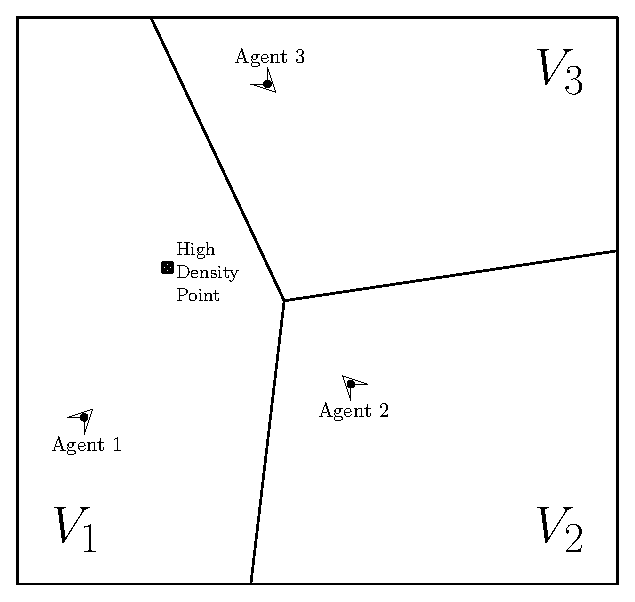
\includegraphics{figs/IPE/voronoiRegions.eps}
    \caption{Plot of agents in their respective Voronoi cells}
    \label{fig:voronoiRegions}
\end{figure}

This square area has been divided up into i Voronoi regions, for i number of agents operating in this area. These regions are represented in figure~\ref{fig:voronoiRegions} as V1, V2, and V3. In our case we are using three agents, though note that this number is somewhat arbitrary and can be scaled to any reasonable number. \\
\\
A Voronoi region is a partition of a plane such that all points within the partition's boundary must be closer to points within its boundary than to points outside. As such, the regions themselves must be convex two dimensional shapes. Therefore, the Voronoi regions represent a specific area covered by each agent within the region. \\
\\ 
The density function itself is applied to each x-y coordinate in the square area. Figure~\ref{fig:contour3Density} shows how a single density region is represented in three-dimensional space.
%\todo[inline]{Add grid to this picture}
\begin{figure} [H]
    \centering
    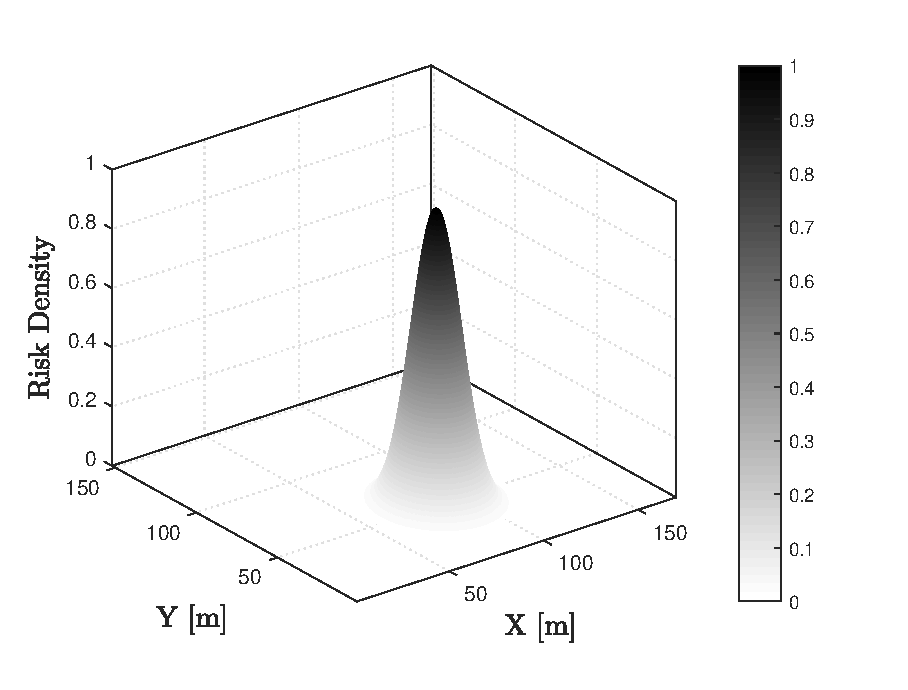
\includegraphics[width=0.8\textwidth]{figs/Matlab/contour3Density.eps}
    \caption{Density distribution centered at point (50,85)m.}
    \label{fig:contour3Density}
\end{figure}

%=========================================================================
Now that we had an idea of the how we would represent density we began looking at we would address the concept of coverage in our system. \\

Dr. Miah provided us with a derivation for coverage that I will detail here. The area coverage metric $H$ in our system for i number of agents is defined as:
\begin{align}
 H = \displaystyle\sum_{i=1}^{n} \int_{V_i} \phi(\mathbf{q}) f(r_{i}^2) \mathrm{d}{\cal Q}   
\end{align}
Where $f(r_{i}^2)$ is a function that models sensor characteristics.
\begin{align}
    f(r_{i}^2) = \alpha*e^{-\beta r_{i}^2}
\end{align}
Note that alpha and beta from the above represent ideal sensor parameters that we are not interested in modelling exactly. Our goal is to find a point in each Voronoi region ${\mathbf{p}}^{[i]}$ such that $H$ is maximized. In order to do such we first find $\frac{\mathrm{d}H}{\mathrm{d}\mathbf{p}^{[i]}}$ and set it to zero. 
\\
For that let us define an individual case:
\begin{align}
    H_{i} = \int_{V_i} \phi(\mathbf{q}) f(r_{i}^2) \mathrm{d}{\cal Q}.
\end{align}
First let us take the derivative:
\begin{align}
    \frac{\mathrm{d}H}{\mathrm{d}\mathbf{p}^{[i]}} = \frac{\mathrm{d}}{\mathrm{d}\mathbf{p}^{[i]}} \displaystyle\sum_{i=1}^{n} H_i = \displaystyle\sum_{i=1}^{n} \int_{V_i} f(r_{i}^2) \phi(\mathbf{q}) \mathrm{d}{\cal Q}
    \label{eq:d_H_4}
\end{align}
As the derivative of the coverage metrics $\displaystyle\sum_{i=1}^{n}H_i$ is zero at all other indices other than the current agent index $i$, we can ignore those values and further simplify Equation~\eqref{eq:d_H_4}.
\begin{align}
    \frac{\mathrm{d}H}{\mathrm{d}\mathbf{p}^{[i]}} = \frac{\mathrm{d}H_i}{\mathrm{d}\mathbf{p}^{[i]}} = \frac{\mathrm{d}}{\mathrm{d}\mathbf{p}^{[i]}} \int_{V_i} f(r_{i}^2) \phi(\mathbf{q}) \mathrm{d}{\cal Q} = \int_{V_i} \frac{\mathrm{d}f({r_i}^2)}{\mathrm{d}{r_i}^2} \frac{\mathrm{d}{r_i}^2}{\mathbf{p}^{[i]}} \phi(\mathbf{q})\mathrm{d}{\cal Q}
    \label{eq:d_H_5}
\end{align}
After the algebraic manipulation of derivative variables, note that we can find the derivative of the introduced range:
\begin{align}
    \frac{\mathrm{d}{r_i}}{\mathrm{d}\mathbf{p}^{[i]}} = \frac{\mathrm{d}}{\mathrm{d}\mathbf{p}^{[i]}}\sqrt{(x-{x}^{[i]]})^2 + (y-{y}^{[i]]})^2}
    \label{eq:d_ri_6}
\end{align}
The function is then squared in order to simplify the derivative calculation:
\begin{align}
    \frac{\mathrm{d}{{r_i}^2}}{\mathrm{d}\mathbf{p}^{[i]}} = \frac{\mathrm{d}}{\mathrm{d}\mathbf{x}^{[i]}\mathrm{d}\mathbf{y}^{[i]}}[(x-{x}^{[i]})^2 + (y-{y}^{[i]})^2] = (-2x+{x}^{[i]}) + (-2y+{y}^{[i]}) = -2(\mathbf{q} - \mathbf{p}^{[i]})
    \label{eq:d_ri2_7}
\end{align}
Using Equations~\eqref{eq:d_ri_6} and \eqref{eq:d_ri2_7}, we are able to simplify Equation~\eqref{eq:d_H_5} even further:
\begin{align}
    \frac{\mathrm{d}H}{\mathrm{d}\mathbf{p}^{[i]}} = \int_{V_i} [-2 \phi(\mathbf{q}) \frac{\mathrm{d}f}{\mathrm{d}{r_i}^2}](\mathbf{q} - \mathbf{p^{[i]}}) \mathrm{d}{\cal Q}
    \label{eq:d_H_8}
\end{align}
The quantity $[-2 \phi(\mathbf{q}) \frac{\mathrm{d}f}{\mathrm{d}{r_i}^2}]$ shown in Equation~\eqref{eq:d_H_8} is introduced as the modified $\phi(\mathbf{q})$ function. This function takes into account the sensor parameters. We call this new function $\Tilde{\phi}(\mathbf{q},\mathbf{p}^{[i]})$. From Equation~\eqref{eq:d_H_8}:
\begin{align}
    \frac{\mathrm{d}H}{\mathrm{d}\mathbf{p}^{[i]}} = \int_{V_i} \Tilde{\phi}(\mathbf{q},\mathbf{p}^{[i]}) (\mathbf{q} - \mathbf{p}^{[i]}) \mathrm{d}{\cal Q}
    \label{eq:d_H_9}
\end{align}
Using properties of integrals, we split the integral into two:
\begin{align}
    \frac{\mathrm{d}H}{\mathrm{d}\mathbf{p}^{[i]}} = \int_{V_i} \mathbf{q} \Tilde{\phi}(\mathbf{q},\mathbf{p}^{[i]}) \mathrm{d}{\cal Q} - \mathbf{p}^{[i]} \int_{V_i} \Tilde{\phi}(\mathbf{q},\mathbf{p}^{[i]}) \mathrm{d}{\cal Q}
    \label{eq:d_H_10}
\end{align}
Finally, we make an algebraic substitution and compare this equation to the mass and centroid equations previously discussed:
\begin{align}
    \frac{\mathrm{d}H}{\mathrm{d}\mathbf{p}^{[i]}} = \int_{V_i} \Tilde{\phi}(\mathbf{q},\mathbf{p}^{[i]}) \mathrm{d}{\cal Q} \frac{\int_{V_i} \mathbf{q} \Tilde{\phi}(\mathbf{q},\mathbf{p}^{[i]}) \mathrm{d}{\cal Q}}{\int_{V_i} \Tilde{\phi}(\mathbf{q},\mathbf{p}^{[i]}) \mathrm{d}{\cal Q}} - \mathbf{p}^{[i]} \int_{V_i} \Tilde{\phi}(\mathbf{q},\mathbf{p}^{[i]}) \mathrm{d}{\cal Q}
    \label{eq:d_H_11}
\end{align}
We know that the mass is defined as the integral of our density function relative to a bounded area $V_i$. As such the modified mass is expressed as $\Tilde{M_{V_i}} =  \int_{V_i} \Tilde{\phi}(\mathbf{q},\mathbf{p}^{[i]}) \mathrm{d}{\cal Q}$. The modified centroid is expressed as any point within the bounded area scaled by our modified $\Tilde{\phi}(\mathbf{q},\mathbf{p}^{[i]})$ function. We call it $\Tilde{C_{V_i}} = \frac{\int_{V_i} \mathbf{q} \Tilde{\phi}(\mathbf{q},\mathbf{p}^{[i]}) \mathrm{d}{\cal Q}}{\int_{V_i} \Tilde{\phi}(\mathbf{q},\mathbf{p}^{[i]}) \mathrm{d}{\cal Q}}$.
\\
Therefore we can express:
\begin{align}
    \frac{\mathrm{d}H}{\mathrm{d}\mathbf{p}^{[i]}} = \Tilde{M_{V_i}} \Tilde{C_{V_i}}-\mathbf{p}^{[i]} \Tilde{M_{V_i}} = 0 \\
    \Tilde{M_{V_i}}(\Tilde{C_{V_i}} - \mathbf{p}^{[i]}) = 0 \\
    \Tilde{C_{V_i}} = \mathbf{p}^{[i]}
\end{align}
In conclusion, as the mass can not be zero, the coverage is maximized when the position of the agent is equal to the modified centroid of a bounded area.



\section{Introduction}
\label{sec:introAreaCoverageModeling}

\section{Conclusion}
\label{sec:conclusionAreaCoverageModeling}

\input{parts/30-MAFOSS.tex}
\input{parts/40-SimulationResults}
\input{parts/50-ExperimentalResults.tex}
\input{parts/60-Conclusion.tex}

% %----------------------------------------------------------------------
% % APPENDICES
% %---------------------------------------------------------------------- 
% \appendix
% % Designate with \appendix declaration which just changes numbering style 
% % from here on
% % Add a title page before the appendices and a line in the Table of Contents
\chapter*{APPENDICES}
\addcontentsline{toc}{chapter}{APPENDICES} 

% An appendix
%======================================================================
\chapter{Implementation Appendix}
\label{ch:Implement-Appendix}
%======================================================================


\section{Downloading image onto the Beaglebone Blue}

\section{Building the eduMOD robot}

\section{Installing ROS on the image}

\section{Setting up the network}



%%% Local Variables:
%%% mode: latex
%%% TeX-master: "../finalReportMainV1"
%%% End:
 	%
% Implementation Code appendix
%======================================================================
\chapter{Implementation Code}
\label{ch:Appendix-Implementation-Code} 
%======================================================================
\section{Local Control Code}


\begin{mdframed}[backgroundcolor=yellow!5, roundcorner=10pt,outerlinecolor= blue!70!black,outerlinewidth=1.2,frametitle=Test code.c]
\inputminted[linenos=true]{c}{code/CCode/test.c}
\end{mdframed}


\section{Matlab Code for Line Follower}

\section{Matlab Code for Leader Follower}

\section{Matlab Code for Area Coverage Optimization}


%%% Local Variables:
%%% mode: latex
%%% TeX-master: "../finalReportMainV1"
%%% End:
 % Code used in implementation

% An appendix
%======================================================================
\chapter{Simulation Appendix}
\label{ch:Appendix-Simulation} 
%======================================================================
\section{Downloading VREP-ROS on Linux}

\section{Setting up network on VREP}

\section{Creating and Modelling the eduMOD robot in VREP-ROS}

\section{Creating the workspace} 


%%% Local Variables:
%%% mode: latex
%%% TeX-master: "../finalReportMainV1"
%%% End:
	%
% Simulation Code appendix
%======================================================================
\chapter{Simulation Code}
\label{ch:Appendix-Simulation-Code} 
%======================================================================
\section{LUA Script used to communicate via ROS}


%%% Local Variables:
%%% mode: latex
%%% TeX-master: "../finalReportMainV1"
%%% End:
 % Code used in simulation

% An appendix
%======================================================================
\chapter{Modelling}
\label{ch:Appendix-Modelling} 
%======================================================================
\section{Matlab Code}

\section{Math and Voronoi stuff not explained in paper?} 

%%% Local Variables:
%%% mode: latex
%%% TeX-master: "../finalReportMainV1"
%%% End:
		% Matlab modelling etc...


% %----------------------------------------------------------------------
% % END MATERIAL
% %----------------------------------------------------------------------

% % B I B L I O G R A P H Y
% % -----------------------
% %
% The following statement selects the style to use for references.  It controls the sort order of the entries in the bibliography and also the formatting for the in-text labels.
\bibliographystyle{plain}
% This specifies the location of the file containing the bibliographic information.  
% It assumes you're using BibTeX (if not, why not?).
\ifthenelse{\boolean{PrintVersion}}{
\cleardoublepage % This is needed if the book class is used, to place the anchor in the correct page,
                 % because the bibliography will start on its own page.
}{
\clearpage       % Use \clearpage instead if the document class uses the "oneside" argument
}
\phantomsection  % With hyperref package, enables hyperlinking from the table of contents to bibliography                        
% % The following statement causes the title "References" to be used for the bibliography section:
% % \renewcommand*{\bibname}{References}
% Bibliography 
\renewcommand{\bibname}{Bibliography}

% Add the References to the Table of Contents
\addcontentsline{toc}{chapter}{\textbf{References}}

\bibliography{bib/refsMultiAgent,bib/seniorProject2-2018,bib/refsSuruzWeb,bib/refsBooksTRTheses}
% Tip 5: You can create multiple .bib files to organize your references. 
% Just list them all in the \bibliogaphy command, separated by commas (no spaces).


%----------------------------------------------------------------------
\end{document}
%======================================================================



%%% Local Variables: 
%%% mode: latex
%%% TeX-master: t
%%% End: 
